\documentclass[serif,9pt]{beamer}
\usepackage{color,listings}
\usepackage{ragged2e}
\usepackage[spanish]{babel}
\usepackage[utf8]{inputenc}
\usepackage{graphicx}

\definecolor{dkgreen}{rgb}{0,0.6,0}
\definecolor{gray}{rgb}{0.5,0.5,0.5}
\definecolor{mauve}{rgb}{0.58,0,0.82}
\definecolor{lgray}{rgb}{0.99,0.97,0.95}
\newcommand{\X}{\textbf{X}}
\newcommand{\Y}{\textbf{Y}}
\newcommand{\Z}{\textbf{Z}}
\newcommand{\G}{\textbf{G}}
\newcommand{\R}{\textbf{R}}
\newcommand{\V}{\textbf{V}}
\newcommand{\Q}{\textbf{Q}}
\newcommand{\h}{\textbf{H}}
\newcommand{\T}{\textbf{T}}

\def\E{\mathbb{E}}
\def\C{\mathbb{C}}
\def\N{\mathbb{N}}

\setbeamercovered{transparent}


\usetheme{Frankfurt}
%\usecolortheme{rose}
%\usecolortheme{lily}
\usepackage{amsmath, multirow}
%\usepackage{color, amsmath, wrapfig, anysize, graphicx, hyperref, amsthm, fancyhdr, amssymb,geometry,amsfonts,float}

\newcommand{\ds}{\displaystyle}


\titlegraphic{
\includegraphics[width=4cm]{utfsm.eps}}%
   %\includegraphics[width=4cm]{fig/inria.eps}}

\begin{document}
\title{Presentación de Seminario de Tesis} 
\author[Paulina Silva Ghio]{\textsc{Paulina Silva Ghio} \\ \medskip
\small{}
\medskip
\url{pasilva@alumnos.inf.utfsm.cl}}
\institute[]{}
\date{15-01-2016.}

\begin{frame}[plain]
\titlepage
\end{frame}


\begin{frame}
\frametitle{Indice}
\tableofcontents
\end{frame} 


\section{Introducci\'on}
\subsection{Contexto}
\begin{frame}
\frametitle{Contexto}

	\begin{itemize}
		\item La guerra de los Navegadores: construir y parchar.
		\item El navegador web: herramienta de uso cotidiano.
		\item El usuario com\'un utiliza servicios.
		\item Distintos tipos, distintas implementaciones.
		\item Web 2.0 y 3.0: AJAX (Asynchronous Javascript and XML).
	\end{itemize}
\end{frame}


\begin{frame}
\frametitle{Browser en la Actualidad}
	\begin{figure}[h]
	    \centering
	    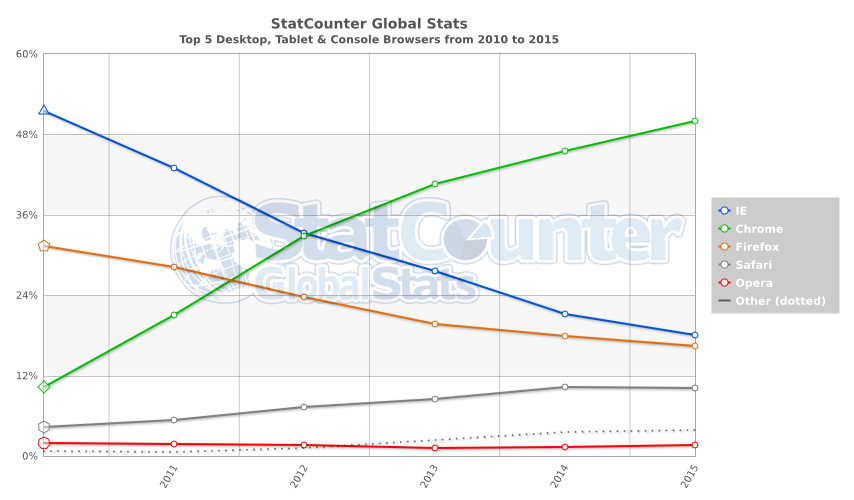
\includegraphics[width=1\textwidth]{figures/StatCounter-browser-ww-yearly-2010-2015.png}
	    \caption{Porcentaje de uso de Navegadores. Fuente: \cite{statBrow}}
	    \label{fig:UsageShare}
	\end{figure}
\end{frame}

\begin{frame}
	\frametitle{El Problema...}
	\begin{itemize}
		\item Sistemas actuales son muy complejos.
		\item Es necesario utilizar metodologías que aseguren: Requerimientos Funcionales y No-Funcionales.
		\item Defectos y errores en el Software generan vulnerabilidades.
		\item La Seguridad es un costo ``extra", a veces no considerado.
	\end{itemize}
	\begin{block}{Las vulnerabilidades...}
		Ocurren por que no se ha tomado en cuenta la seguridad en el desarrollo.
	\end{block}
\end{frame}


\subsection{Seguridad...}
\begin{frame}
\frametitle{Seguridad...}
	\begin{block}{Desde la perspectiva de seguridad \cite{WhyteHarrison}:}
		\begin{itemize}		
			\item ¿Qu\'e realizan las universidades o la industria?
			\item Proyectos de desarrollo de software, ¿cuanto se le dedica a la seguridad?
			\item ¿La industria asegura que los sistemas a construir, sean seguros?
		\end{itemize}
	\end{block}
	\begin{block}{¿Qu\'e conceptos de seguridad sabe en promedio un estudiante graduado de carrera relacionada a Computer Science?}
		\begin{itemize}
			\item ¿La gente es autodidacta? o ¿aprende por necesidad?
			\item ¿La malla curricular es suficiente?
		\end{itemize}
	\end{block}
\end{frame}


\subsection{Desarrollo de Software y Seguridad}
\begin{frame}
\frametitle{Desarrollo de Software y Seguridad}
	\begin{itemize}
		\item ¿Qu\'e tanto se diferencian las preocupaciones del usuario com\'un y el desarrollador que crea los sistemas?
		\item ¿C\'omo desarrollar software seguro?
	\end{itemize}
	\begin{block}{Construcci\'on de Software Seguro...}
		\begin{itemize}
			\item Los que participan en la construcci\'on: deben entender los problemas de seguridad.
			\item No basta saber como est\'a construido.
			\item Considerar la Seguridad desde el inicio del Proyecto.
			\item Seguridad como una Propiedad Sist\'emica.
		\end{itemize}
	\end{block}
\end{frame}


\subsection{Motivaci\'on para estudiar el Browser}
\begin{frame}
	\frametitle{Motivaci\'on para estudiar el Browser}
	\onslide{El browser es una herramienta indispensable, \'este permite:}
	\begin{itemize}
		\item Nuevas formas de interactuar.
		\item Disminuir los costos de construir un programa Cliente (desde cero) para
el usuario del sistema.
		\item Seguridad (la que est\'a implementada en los Web Browser es bastante buena).
		\item Es una herramienta indispensable, por lo tanto el reuso es lógico.
	\end{itemize}
	
	\begin{block}{Las preocupaciones principales}
	\begin{itemize}
		\item Los sistemas, a los que un usuario hace referencia, son llamados desde un Web Browser.
		\item Los stakeholders afectados: el usuario del Browser, el Host del usuario y hasta el Servicio extero usado.
		\item Falta de conocimientos de seguridad con respecto al Browser, podr\'ia afectar de forma directa el desarrollo de aplicaciones que lo utilizan y Stakeholders.
	\end{itemize}
	\end{block}
\end{frame}


\subsection{Contribuciones}
\begin{frame}
	\frametitle{Contribuciones}
	\begin{block}{Objetivo General}
		\begin{itemize}
			\item Generar un cuerpo organizado de informaci\'on sobre el Web Browser y su seguridad.
			\item Sistematizar, organizar y clasificar el conocimiento adquirido en un documento, con formato semi-formal.Dado que hay conceptos poco claros y poca documentación formal.
			\item Para: profesionales como Estudiantes del \'area Inform\'atica que est\'en insertos en el \'area de Desarrollo de Software.
		\end{itemize}
	\end{block}
\end{frame}

\begin{frame}
	\frametitle{Contribuciones}
	\begin{block}{Objetivos Espec\'ificos}
		\begin{itemize}
			\item Comprender los conceptos relacionados al navegador web, sus componentes, interacciones o formas de comunicaci\'on, amenazas y ataques a los que puede estar sometido, como tambi\'en los mecanismos de defensa. Esto se realizar\'a a trav\'es del desarrollo de un Estado del Arte sobre el Browser.
			\item Identificar actores, componentes, funciones, relaciones, requerimientos y restricciones del navegador, para lograr abstraer una Arquitectura de Referencia (AR) a partir de documentaci\'on disponible en Internet, blogs de desarrolladores, papers e iniciar un pequeño cat\'alogo de Patrones de Mal Uso. 
			\item Condensar el conocimiento obtenido en el punto anterior a trav\'es de documentos semi-formales.
			\item Una gu\'ia para comunicar los conceptos relevantes que pudieran afectar la relaci\'on existente entre un desarrollo de software y el navegador.
			\item Profundizar el conocimiento en ataques relacionados con m\'etodos de Ingenier\'ia Social.
		\end{itemize}
	\end{block}
\end{frame}

% \begin{frame}
% 	\frametitle{Metodología basada en Fernandez \cite{braz2008eliciting,fernandez2013security}}
% 	\begin{block}{Arquitectura de Referencia (AR)}
% 		\begin{itemize}
% 			\item Especifica la decomposici\'on del sistema en subsistemas, las interacciones entre estas partes y la distribuci\'on de funcionalidad entre ellas.
% 			\item Capturar la esencia de la arquitectura a trav\'es de una colecci\'on de sistemas similares, por medio del reuso arquitect\'onico
% 			\item Ayudar a los implementors o desarrolladores del software, a entender los trade-off cuando se diseñan nuevos sistemas
% 			\item Ayudar a los mantenedores de estos sistemas a entender el c\'odigo legacy usado.
% 			\item Comparar las diferencias en decisiones de diseño y poder entender los cambios realizados a lo largo del Desarrollo de un sistema.
% 			\item Mirada hol\'istica del Sistema.
% 		\end{itemize}
% 	\end{block}
% 	\begin{block}{Patrones del Mal Uso}
% 		\onslide{Permitir\'an enseñar y comunicar las posibles formas en que tal sistema puede ser usado inapropiadamente.}
% 	\end{block}
% \end{frame}

\section{Marco Te\'orico de un Browser}
\begin{frame}
	\frametitle{Marco Te\'orico de un Browser}
	\begin{itemize}
		\item Arquitectura cliente/servidor
		\item Comunicaci\'on e Informaci\'on de estado: HTTP y canales.
		\item SSL/TLS
		\item HTML5 y XML (Markup Languages)
		\item CSS
		\item DOM
		\item Javascript (ECMAScript)
		\item Geolocalizaci\'on, WebWorkers y otros...
	\end{itemize}
	\begin{block}{Desaf\'ios del navegador}
		\begin{itemize}
			\item Contenido y compatibilidad
			\item Navegaci\'on personalizada
			\item Navegaci\'on sin inconvenientes
			\item Seguridad
		\end{itemize}
	\end{block}
\end{frame}

\begin{frame}
	\frametitle{Arquitectura de Referencia (AR)}
	\begin{itemize}
		\item Describir los Stakeholders que interactuan con el sistema y que poseen preocupaciones/concerns de \'este.
		\item Patrones de Arquitectura.
		\item Atributos de calidad deseables que el sistema debe garantizar. Es importante solo destacar aquellos realmente necesarios, dado que un sistema sobrecargado con ellos tampoco es conveniente.
		\item Actualmente no hay un consenso de cómo definir una AR, lo que debería contener y cómo debería de construirse.
	\end{itemize}
	\begin{block}{Ventajas}
		\begin{itemize}
			\item Comprender la estructura subyacente de un Web Browser y las interacciones que tendr\'a con otros sistemas.
			\item Proveer una base tecnol\'ogica modular y flexible. Al tener los subsistemas compartimentalizados es posible quitar y sacar piezas, que poseen interfaces similares, y de esa manera reusar lo otro sin tener que construir un sistema nuevo.
			\item Entrega una base para el desarrollo de otros Navegadores Web, sin explicar detalles de implementaci\'on.
		\end{itemize}
	\end{block}
\end{frame}

\begin{frame}
	\frametitle{Arquitectura de Referencia de Seguridad (ARS)}
	\begin{itemize}
		\item asdf
		
	\end{itemize}
	\begin{block}{Ventajas}
		\begin{itemize}
			\item asdf
		\end{itemize}
	\end{block}
\end{frame}

% \section{(In)Seguridad en el Browser}
% \begin{frame}
% 	\frametitle{Social Engineering Attacks o Ataques de Ingenier\'ia Social: Phishing}
% 	\begin{figure}[h]
%         \centering
%         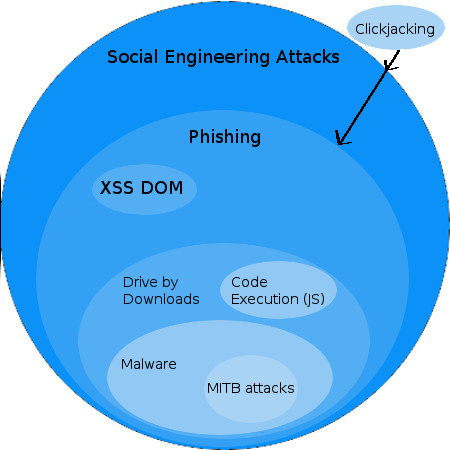
\includegraphics[scale=0.4]{figures/SEAttacks.jpg}
%         \caption{Esquematizaci\'on de ataques de tipo Social Engineering.}
%         \label{fig:SEattack}
%     \end{figure}
% \end{frame}

% \begin{frame}
% 	\frametitle{Instalaci\'on de Malware o extensiones maliciosas}
% 	\begin{figure}[h]
%         \centering
%         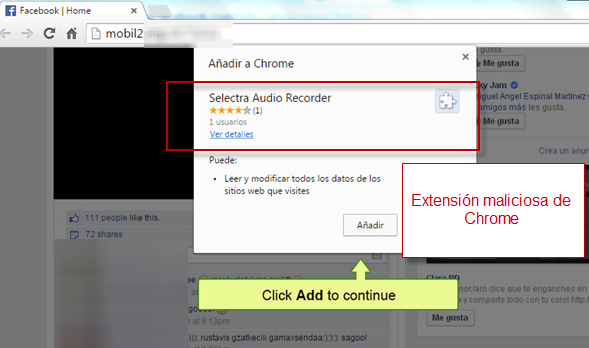
\includegraphics[scale=0.4]{figures/fbporn3.png}
%         \caption{Fijarse en la barra de direcciones, para la p\'agina que supuestamente es Facebook.}
%         \label{fig:Malware}
%     \end{figure}
% \end{frame}

% \begin{frame}
% 	\frametitle{Extensiones Vulnerables}
% 	\begin{figure}[h]
%         \centering
%         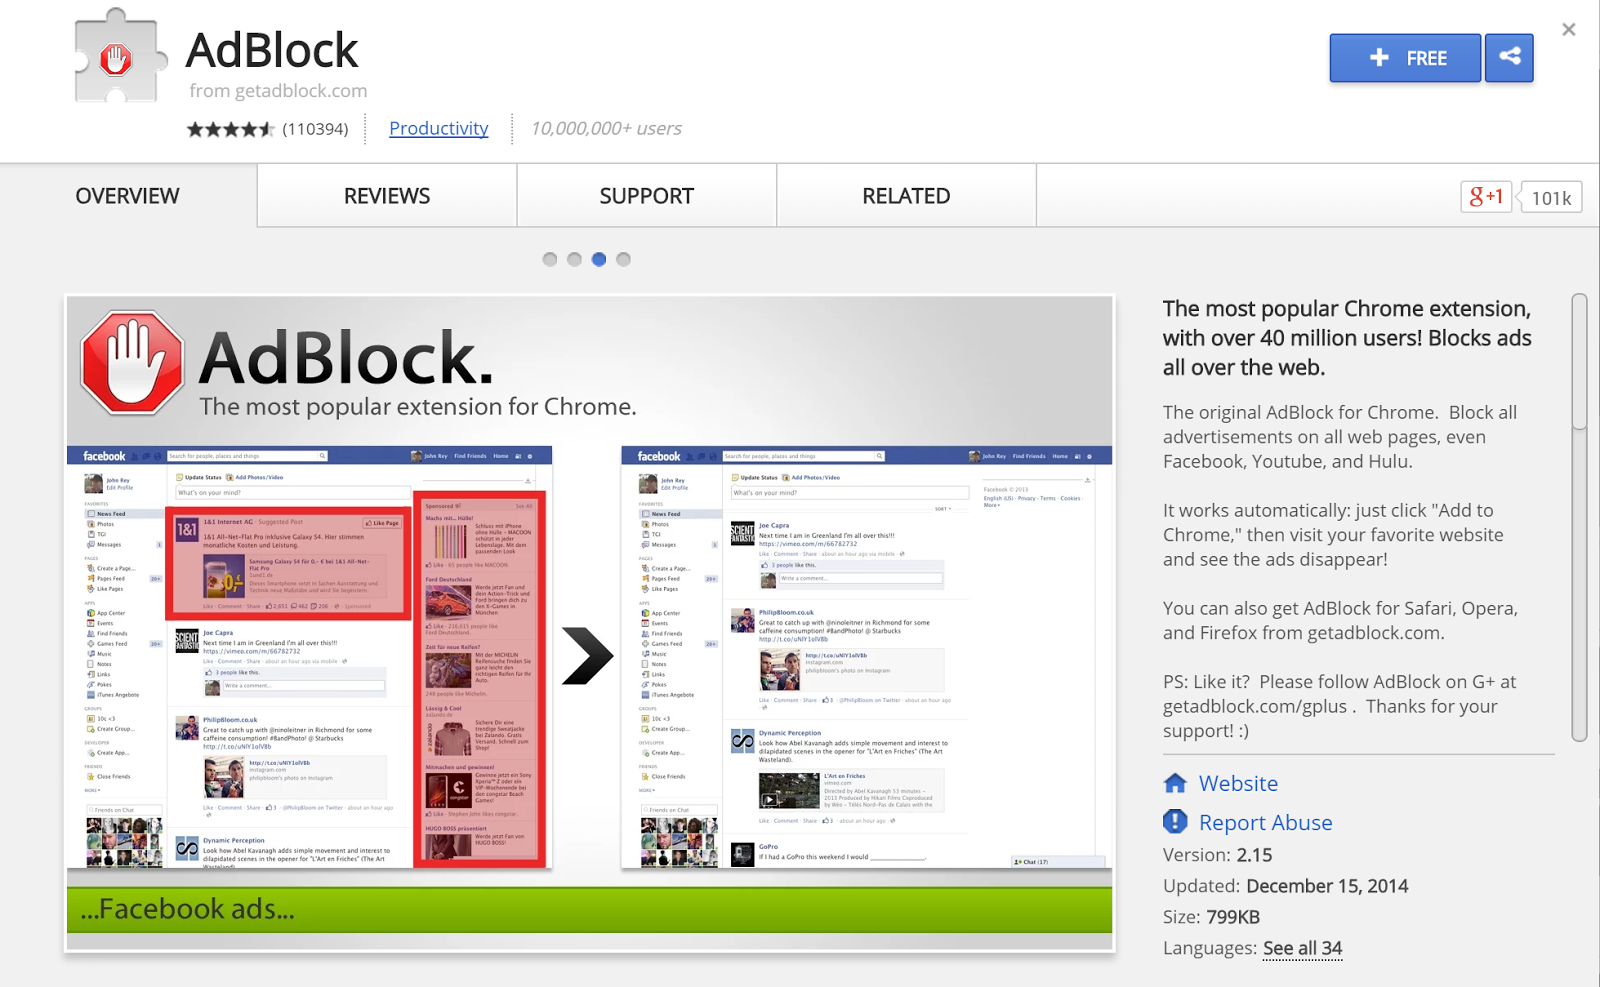
\includegraphics[scale=0.15]{figures/Adblock.png}
%         \caption{¿Qu\'e suceder\'ia si una extensi\'on, confiable para los usuarios, permitiera generar ataques?}
%         \label{fig:vulnExt}
%     \end{figure}
% \end{frame}

% \begin{frame}
% 	\frametitle{Ejecuci\'on de c\'odigo Javascript y XSS-DOM}
% 		\begin{itemize}
% 			\item Ambos generan cambios en el DOM, pero de diferentes maneras (Uno es una especializaci\'on).
% 			\item La ejecuci\'on de javascript podr\'ia pasar ciertos controles de acceso (Javascript Capabilities).
% 			\item Puede terminar realizando conexiones con servidores maliciosos, sin que el usuario se de cuenta (XHR).
% 			\item El DOM puede ser modificado, de tal manera de engañar al usuario.
% 			\item XSS-DOM, el c\'odigo al lado del cliente se ejecuta de una manera distinta dada las modificaciones maliciosas que se han hecho al DOM.
% 		\end{itemize}
% \end{frame}

% \begin{frame}
% 	\frametitle{Man-in-the-Browser}
% 	\begin{figure}[h]
%         \centering
%         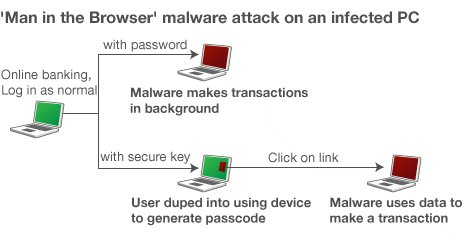
\includegraphics[scale=0.7]{figures/_58291188_malware_464v2.jpg}
%         \caption{Normalmente el ataque se realiza cuando el usuario ha permitido la instalaci\'on en el Host de un ente malicioso: extensi\'on o programa}
%         \label{fig:vulnExt}
%     \end{figure}
% \end{frame}

% \subsection{Mecanismos de Defensa}
% \begin{frame}
% 	\frametitle{Mecanismos de Defensa}
% 	\begin{itemize}
% 		\item SOP o Same Origin Policy
% 		\item CORS o Cross-Origin Resource Sharing
% 		\item HTTP Fields o Campos HTTP
% 		\item Sandboxing: Google Chrome/Chromium e Internet Explorer
% 		\item Aislaci\'on de Contenido
% 		\item Blacklist y Whitelist
% 		\item Sistema de Reputaci\'on
% 		\item Actualizaciones peri\'odicas en background
% 	\end{itemize}
% \end{frame}


\section{Estado del Arte}
\begin{frame}
	\frametitle{Estado del Arte}
	\begin{itemize}
		\item No se encontr\'o informaci\'on actualizada sobre una Arquitectura de Referencia del Browser. Hay una \cite{preprint-grosskurth-browser-archevol}, pero es muy antigua.
		\item Poca documentaci\'on y no hay conceptos unificados.
		\item Queda por buscar si existe algo parecido a una ARquitectura de Referencia de Seguridad del Browser.
	\end{itemize}
\end{frame}

\subsection{Google Chrome y Chromium}
\begin{frame}
	\frametitle{Google Chrome y Chromium}
	\begin{figure}[h]
	    \centering
	    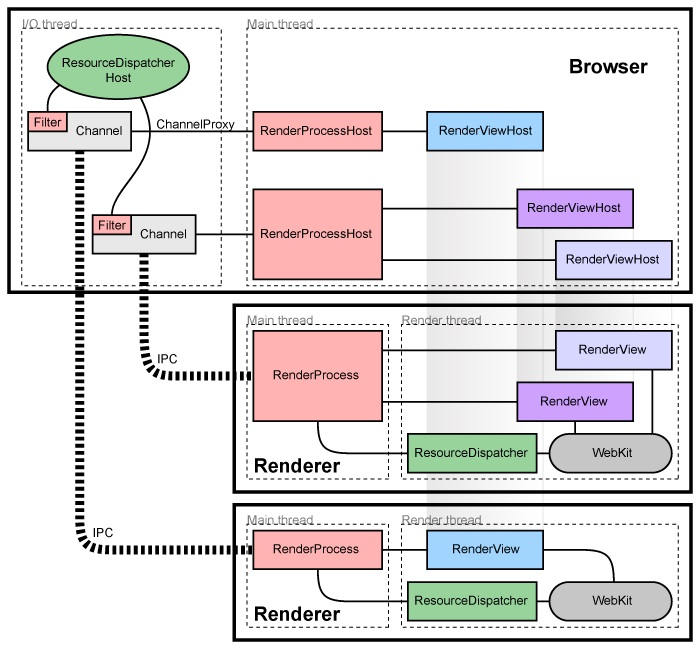
\includegraphics[scale=0.35]{figures/archGC.jpg}
	    \caption{Architectura Multiprocesos de Google Chrome. Fuente: \cite{multiProcGC}}
	    \label{fig:UsageShare}
	\end{figure}
\end{frame}

\begin{frame}
	\frametitle{Google Chrome y Chromium}
	\begin{figure}[h]
        \centering
        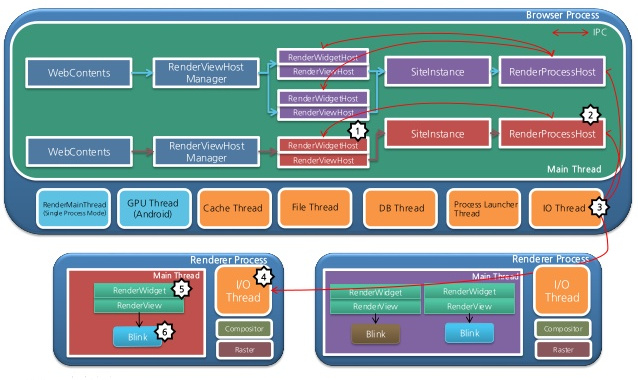
\includegraphics[scale=0.4]{figures/chromium-rendering-pipeline-28-638.jpg}
        \caption{Architectura de Chromium en detalle. Fuente: \cite{ChrRenderPipe}}
        \label{fig:archGC2}
    \end{figure}
\end{frame}

\subsection{Internet Explorer}
\begin{frame}
	\frametitle{Internet Explorer}
	\begin{figure}[h]
	    \centering
		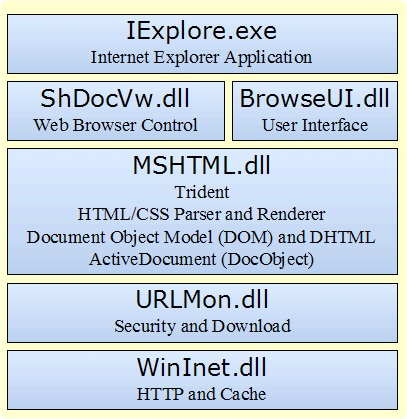
\includegraphics[scale=0.5]{figures/IEArch.jpg}
		\caption{Arquitectura de Internet Explorer. Fuente: \cite{IEArchImg}}
		\label{fig:archIE}
    \end{figure}
\end{frame}

\begin{frame}
	\frametitle{Internet Explorer}
	\begin{figure}[h]
        \centering
        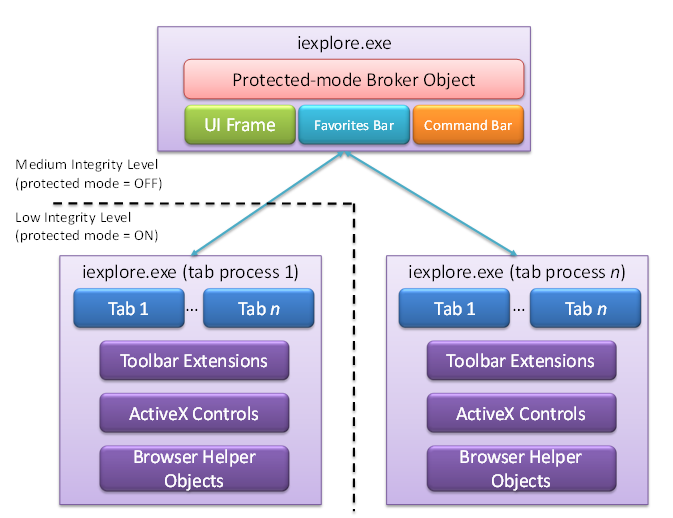
\includegraphics[scale=0.35]{figures/11_IE8andLooselyCoupledIELCIE_2.png}
        \caption{Arquitectura de Internet Explorer m\'as detallada. Fuente: \cite{IE8LCIE}}
        \label{fig:archIE2}
    \end{figure}
\end{frame}

\subsection{Firefox - Electrolysis}
\begin{frame}
	\frametitle{Firefox - Electrolysis}
	\begin{figure}[h]
        \centering
        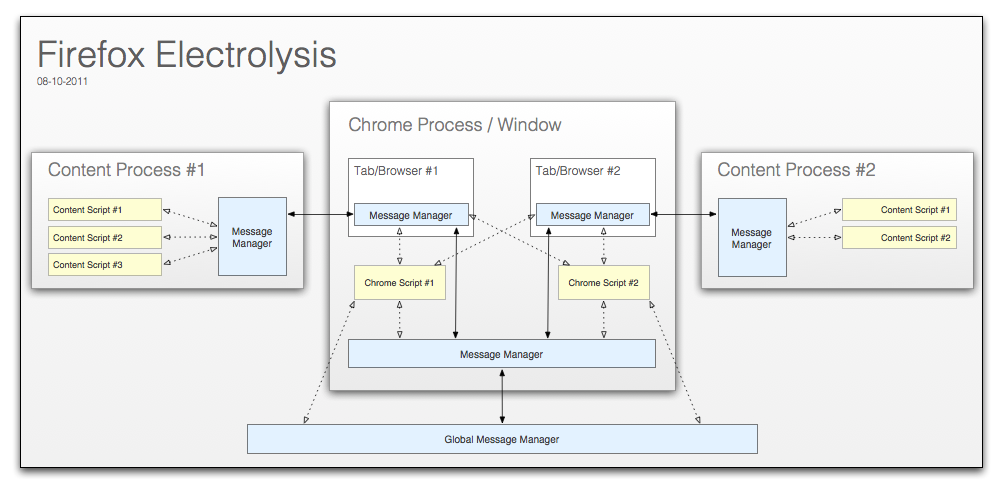
\includegraphics[scale=0.3]{figures/electrolysis.png}
        \caption{Firefox Electrolysis, Comunicaci\'on de procesos 1. Fuente: \cite{Firefox101}}
        \label{fig:ChromePComm1}
    \end{figure}
\end{frame}

\begin{frame}
	\frametitle{Firefox - Electrolysis}
	\begin{figure}[h]
        \centering
        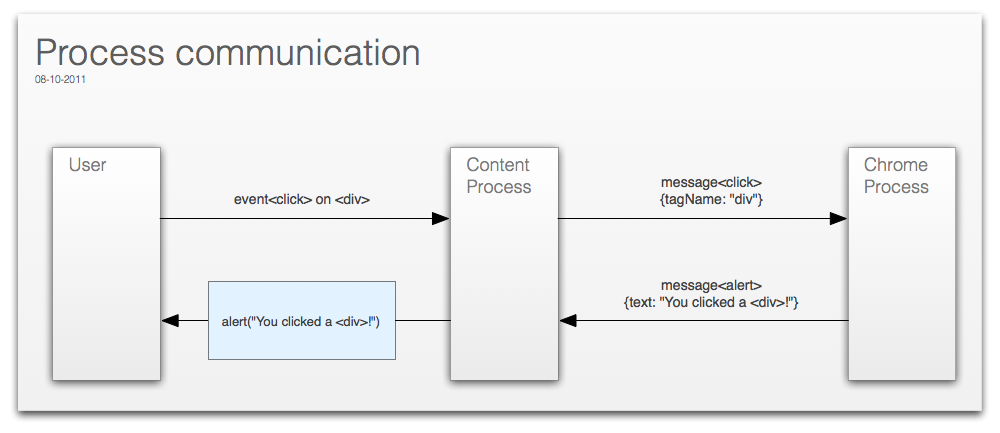
\includegraphics[width=1\textwidth]{figures/e10s-processes.png}
        \caption{Firefox Electrolysis, Comunicaci\'on de procesos 2. Fuente: \cite{Firefox101}}
        \label{fig:ChromePComm2}
    \end{figure}
\end{frame}

% \section{Arquitectura de Referencia}
% \begin{frame}
% 	\frametitle{Casos de Uso}
% 	\begin{figure}[h]
% 	    \centering
% 	    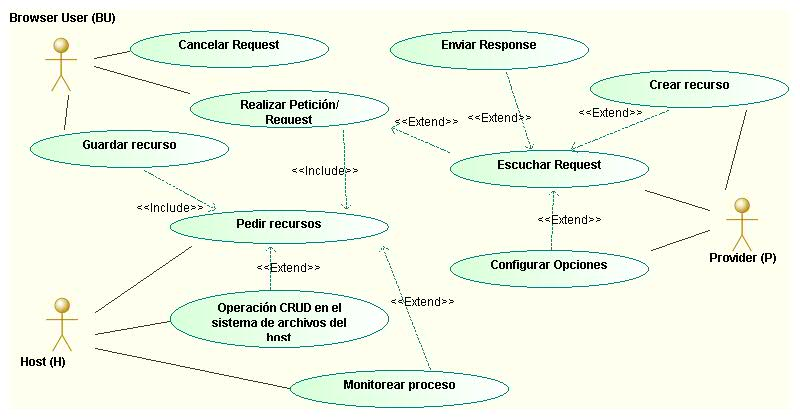
\includegraphics[scale=0.35]{figures/chap4/UCBrowser.jpg}
% 	    \caption{Diagrama de Caso de Uso del \textit{Web Browser}.}
% 	    \label{fig:CUBrowser}
% 	\end{figure}
% \end{frame}

% \begin{frame}
% 	\frametitle{Patr\'on Browser Infrastructure}
% 	\begin{figure}[h]
% 	    \centering
% 	    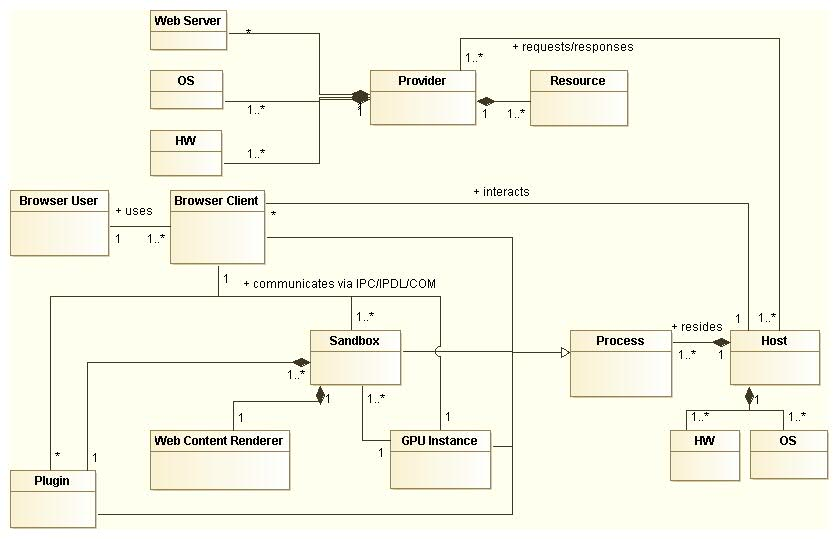
\includegraphics[scale=0.35]{figures/chap4/browserInfraPattern_v3.jpg}
% 	    \caption{Componentes de alto nivel del \textit{Browser}.}
% 	    \label{fig:BIPatt}
% 	\end{figure}
% \end{frame}


% \begin{frame}
% 	\frametitle{Din\'amica: Realizar Request}
% 	\begin{figure}[h]
% 	    \centering
% 	    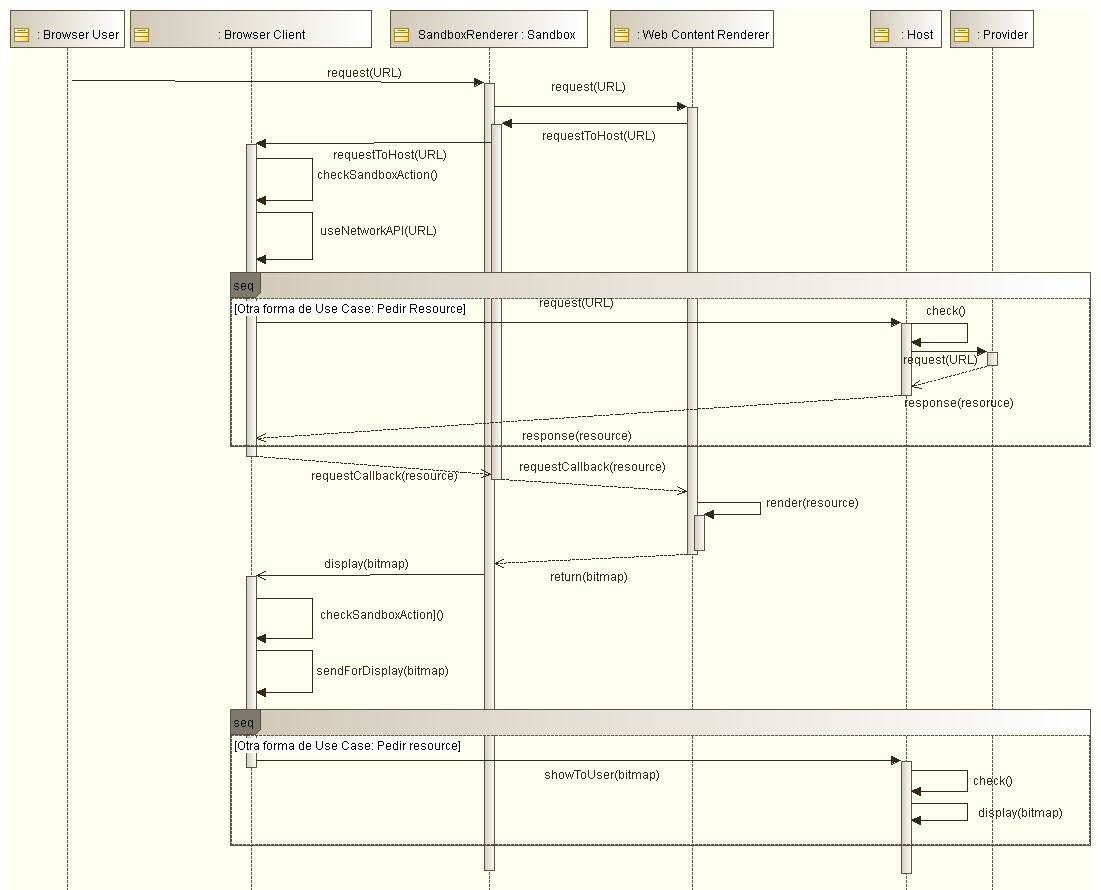
\includegraphics[scale=0.28]{figures/chap4/requestResource_v2.jpg}
% 	    \caption{Diagrama de Secuencia: Realizar Request.}
% 	    \label{fig:SecReq}
% 	\end{figure}
% \end{frame}

% \section{Patr\'on de Mal Uso}
% \begin{frame}
% 	\frametitle{Diagrama de Actividad}
% 	\begin{figure}[h]
% 	    \centering
% 	    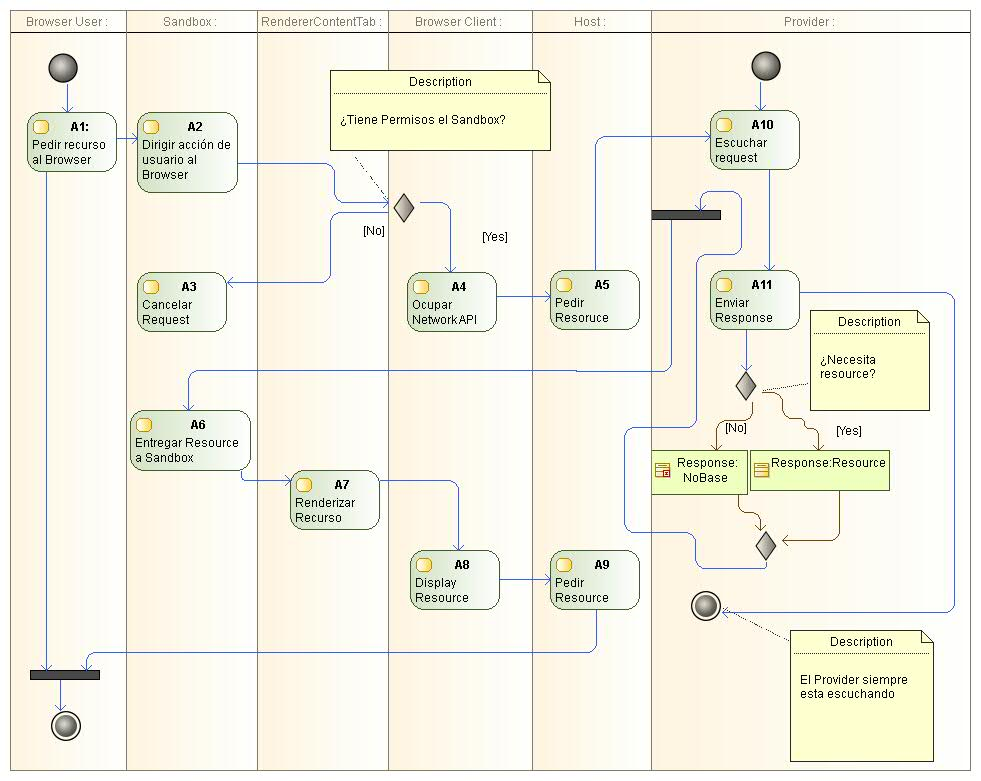
\includegraphics[scale=0.23]{figures/chap5/activityDiag_v3.jpg}
% 	    \caption{Diagrama de Actividad Compuesto para los casos de uso \textbf{Realizar Request} y \textbf{Recibir Request}.}
% 	    \label{fig:ActDiagr}
% 	\end{figure}
% \end{frame}

% \begin{frame}
% 	\frametitle{Diagrama de Clases para el patr\'on de Mal Uso.}
% 	\begin{figure}[h]
% 	    \centering
% 	    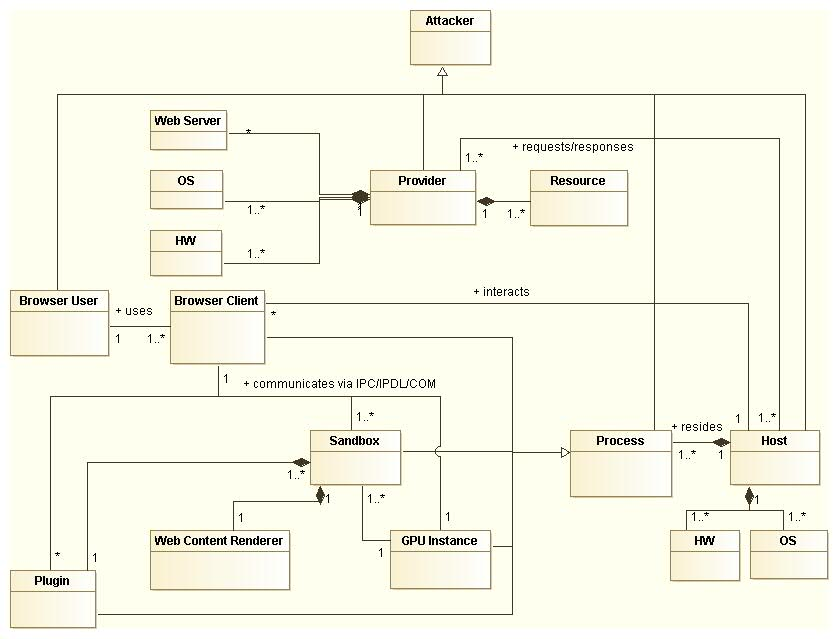
\includegraphics[scale=0.3]{figures/chap5/patronMisuse_v2.jpg}
% 	    \caption{Diagrama de Clases para el patr\'on de Misuse.}
% 	    \label{fig:BIMisuse}
% 	\end{figure}
% \end{frame}

% \begin{frame}
% 	\frametitle{Diagrama de Clases para el patr\'on de Mal Uso.}
% 	\begin{figure}[h]
%         \centering
%         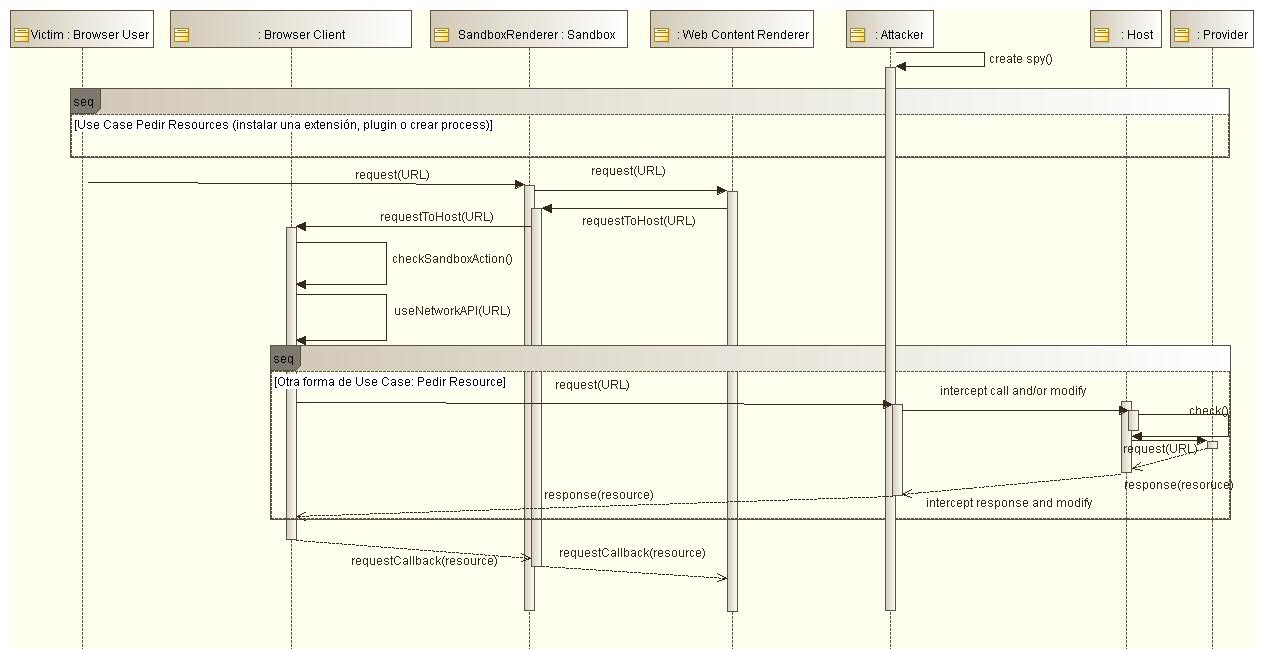
\includegraphics[scale=0.32]{figures/chap5/patronMisuseSeq_v2.jpg}
%         \caption{Diagrama de Secuencia para el Mal uso: Modificaci\'on de tr\'afico en el \textit{Web Browser}.}
%         \label{fig:SeqMisuse}
%     \end{figure}
% \end{frame}


\section{Metodología}
\begin{frame}
	\frametitle{Metodología}
	\begin{itemize}
		\item Marco teórico y Estado del Arte: Revisión de conceptos relevantes del navegador, seguridad y Arquitecturas de Referencias existentes. Se examinarán artículos científicos, blogs o proyectos de investigación relacionados al tema.
		\item Evaluación de Resultados Intermedios: a) Envío de papers a Asian PLoP, b) Depurar el modelo obtenido en la memoria de pregrado.
		\item Agregar nuevos patrones y adecuar modelo para especificar semi-formalmente estos patrones. Creación de la Arquitectura de Referencia de Seguridad.
		\item Producir segunda versión de publicaciones: Se enviarán más trabajos a conferencias de tipo PLoP (Pattern Languages of Programs).
		\item Documentar la tesis a partir de la compilación de papers obtenidos y el trabajo adelantado.
	\end{itemize}
\end{frame}

\section{Plan de Trabajo}
\begin{frame}
	\begin{table}{Plan de Trabajo}
        \begin{tabular}{ m{12em}|m{25em}} 
        \hline        
        \textbf{Actividad} & \textbf{Fecha}\\
        \hline
        Marco teórico y Estado del Arte & Noviembre 2015 - Enero 2016\\
        \hline
        Evaluación de Resultados Intermedios & Noviembre 2015  - Febrero 2016\\
        \hline
        Agregar nuevos patrones y adecuar modelo & Enero - Abril 2016\\
        \hline
        Producir segunda versión de publicaciones & Enero - Abril 2016\\
        \hline
        Documentar la tesis & Enero - Abril 2016\\        
        \hline
        \end{tabular}
        \caption{Plan de Trabajo}
        \label{tab:trabajo}
    \end{table}
\end{frame}

\section{Trabajo Adelantado}
\begin{frame}
	\frametitle{Trabajo Adelantado}
	\begin{itemize}
		\item En la memoria de Pregrado se obtuvo un Estado del Arte sobre el Browser y documentación sobre Arquitecturas de Referencias existntes. Falta averiguar sobre Arquitecturas de Referencia de Seguridad.
		\item Se han enviado 2 papers a la conferencia AsianPLoP con lo obtenido en la memoria de pregrado. El proceso llamado “shepherding” permite evaluar el paper enviado, al mismo tiempo que provee al autor la mejora del trabajo a través del intercambio continuo de sugerencias entre el autor/autores con el “shepherd”.
	\end{itemize}
\end{frame}


\section{Conclusiones}
\begin{frame}
	\frametitle{Conclusiones}
	asasas
\end{frame}

\begin{frame}
	\frametitle{Contribuciones}	
	\begin{itemize}
	\item asadsd
		% \item Base Conceptual: términos de seguridad relacionados al navegador Web.
		% \item Construcción del primer Patrón Arquitectural sobre la infraestructura del Web Browser.
		% \item Una parte de la Arquitectura de Referencia ha sido construída, a través de la abstracción del Patrón Browser Infrastructure.
		% \item Stakeholders y Casos de Uso más importantes
		% \item Patrones de Mal Uso.
	\end{itemize}
\end{frame}

\begin{frame}
	\frametitle{Resumen}	
	\begin{itemize}
		\item asasa
		% \item Una śintesis y abstracción de la información correspondiente a los Web Browsers, para generar un lenguaje de comunicación de los conceptos. El uso de patrones permite ayudar a un conjunto de personas a unificar conceptos, así como también puede ser guía en futuros desarrollos.
		% \item El trabajo propuesto permite comprender mejor, por medio de la Arquitectura de Referencia parcialmente construída, tanto componentes como amenazas existentes. Además como no está sujeto a implementaciones específicas, es posible generalizar ciertos resultados en otros Browsers.
		% \item Comunicar en primera instancia, los conceptos de seguridad básicos para un mejor entendimiento de los subsistemas que interactuan en la Internet. Los patrones de Mal Uso permiten condensar la información y transmitirla, de forma ordenada y descriptiva.
		% \item Entregar el conocimiento básico de los componentes e interacciones entre el Web Browser y un proveedor de recursos externo; así como también de las amenazas que existen
	\end{itemize}
\end{frame}

\begin{frame}
	\frametitle{¿Preguntas?}
	¡Muchas Gracias!	
\end{frame}

\bibliography{refTodas}
\bibliographystyle{IEEEtran}

\end{document}

